% Figura Anexo I: derivación de la curva IS desde el aspa keynesiana (dos paneles apilados)
\documentclass[tikz,border=3pt]{standalone}
\usepackage[T1]{fontenc}
\usepackage[utf8]{inputenc}
\usetikzlibrary{arrows.meta,calc,positioning}
\begin{document}
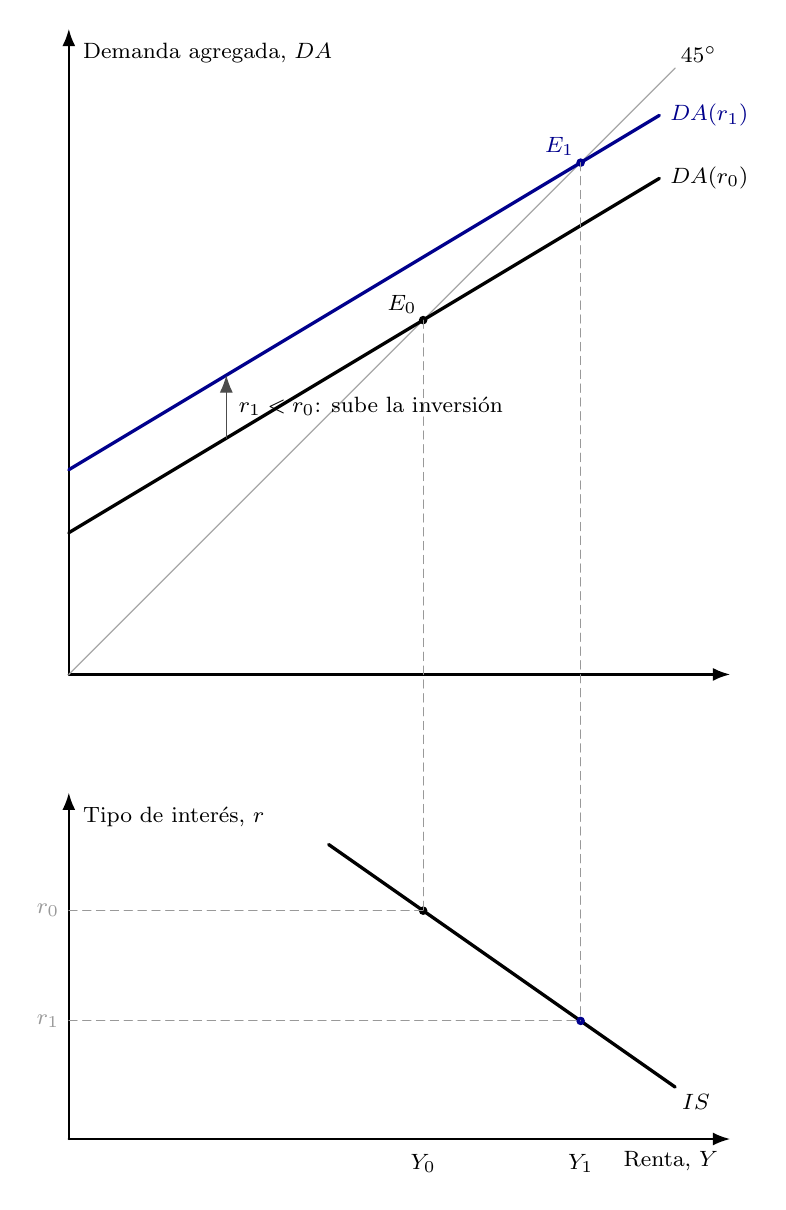
\begin{tikzpicture}[>={Latex[length=2.2mm]}, line cap=round, font=\footnotesize,
  eje/.style={->, thick},
  curva/.style={very thick},
  nueva/.style={very thick, blue!55!black},
  guia/.style={densely dashed, gray!80},
  pto/.style={circle, fill=black, inner sep=1.1pt}]
  % ---------- Panel superior: aspa keynesiana ----------
  \draw[eje] (0,0) -- (8.4,0);
  \draw[eje] (0,0) -- (0,8.2) node[below right=2pt]{Demanda agregada, $DA$};
  \draw[gray!70] (0,0) -- (7.7,7.7) node[above right=-2pt, black]{$45^{\circ}$};
  \draw[curva] (0,1.8) -- (7.5,6.3) node[right]{$DA(r_0)$};
  \draw[nueva] (0,2.6) -- (7.5,7.1) node[right]{$DA(r_1)$};
  \draw[->, gray!60!black] (2.0,3.0) -- (2.0,3.8) node[midway, right=1pt, black]{$r_1<r_0$: sube la inversión};
  \node[pto] (E0) at (4.5,4.5) {};
  \node[above left=0pt of E0, inner sep=1pt] {$E_0$};
  \node[pto, fill=blue!55!black] (E1) at (6.5,6.5) {};
  \node[above left=0pt of E1, inner sep=1pt, blue!55!black] {$E_1$};
  % ---------- Panel inferior: curva IS ----------
  \begin{scope}[yshift=-5.9cm]
    \draw[eje] (0,0) -- (8.4,0) node[below left=1pt]{Renta, $Y$};
    \draw[eje] (0,0) -- (0,4.4) node[below right=2pt]{Tipo de interés, $r$};
    \draw[curva] (3.3,3.74) -- (7.7,0.66) node[below right=-2pt]{$IS$};
    \node[pto] (A) at (4.5,2.9) {};
    \node[pto, fill=blue!55!black] (B) at (6.5,1.5) {};
    \draw[guia] (0,2.9) node[left]{$r_0$} -- (4.5,2.9);
    \draw[guia] (0,1.5) node[left]{$r_1$} -- (6.5,1.5);
    \node[below=2pt] at (4.5,0) {$Y_0$};
    \node[below=2pt] at (6.5,0) {$Y_1$};
  \end{scope}
  % Guías verticales entre paneles
  \draw[guia] (4.5,4.5) -- (4.5,-3.0);
  \draw[guia] (6.5,6.5) -- (6.5,-4.4);
\end{tikzpicture}
\end{document}
